\documentclass[]{gshs_exam_S}

\usetikzlibrary{patterns,decorations.pathmorphing,arrows.meta}
\usepackage{bm}

\usepackage{tikz-3dplot}


\makeatletter
\myyear{2018}\let\MyYear\@myyear %학년도
\semester{1}\let\Semester\@semester %학기
\exams{1차 지필평가}\let\Exams\@exams %1차,2차 지필평가
\subject{물리학세미나I}\let\Subject\@subject %과목명
\credits{2} %학점
\pfscore{100} %만점
\examtime{60분} %시험시간
\examiner{목진욱} %출제
\reviewer{안재훈} %검토
\makeatother

%% 한글줄간격 %%
\renewcommand{\baselinestretch}{1.3}

\begin{document}

\maketitle

%%% page 1 %%%
\begin{multicols*}{2}
\noindent\fbox{\parbox{0.98\columnwidth}{\vspace*{-0.6em}
\begin{enumerate}[leftmargin=5.5mm,label=※]
\item 문항에 따라 배점이 다르므로 각 물음의 끝에 표시된 배점을 참고하시오.\\[-2.2em]
\item 서술형 ( 80 )점 포함, 논술형 ( 20 )점 포함
\end{enumerate}\vspace{-0.6em}}}\vspace{1em}

\begin{questions}
\extrawidth{8.1em}
%%% Problem 1 %%%
\question[10] \ssh\ 그림과 같이 질량이 각각 $1\,\mathrm{kg}$, $5\,\mathrm{kg}$, $5\,\mathrm{kg}$, $24\,\mathrm{kg}$인 네 개의 추들이 도르래를 걸쳐 실로 연결되어 있다. 맨 위 도르래에 $F=240\,\mathrm{N}$의 힘이 연직 상방으로 작용할 때, 맨 위 도르래의 가속도를 구하시오. 단, 도르래들과 실의 잘량은 무시하고, 마찰은 없으며, 중력가속도는 $g=10\,\mathrm{m/s^2}$으로 가정한다.\droppoints \begin{center}
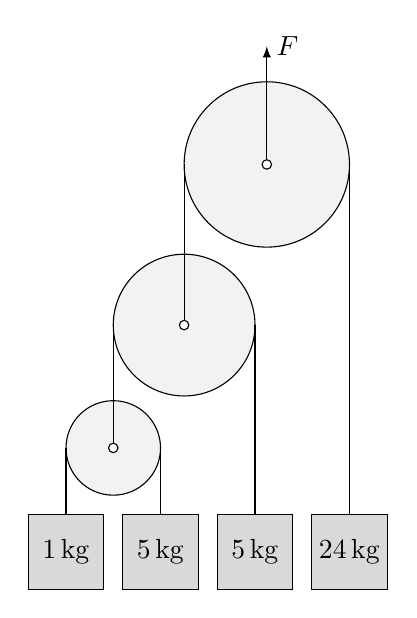
\begin{tikzpicture}
\def\r{0.6}
\draw[fill=black!15] (0,0) rectangle ({1.6*\r},{1.6*\r}) node[pos=0.5]{$1\,\mathrm{kg}$};
\draw[fill=black!15] ({2*\r},0) rectangle ({3.6*\r},{1.6*\r}) node[pos=0.5]{$5\,\mathrm{kg}$};
\draw[fill=black!15] ({4*\r},0) rectangle ({5.6*\r},{1.6*\r}) node[pos=0.5]{$5\,\mathrm{kg}$};
\draw[fill=black!15] ({6*\r},0) rectangle ({7.6*\r},{1.6*\r}) node[pos=0.5]{$24\,\mathrm{kg}$};
\draw[fill=black!5] ({1.8*\r},{3*\r}) circle (\r);\draw[fill=white] ({1.8*\r},{3*\r}) circle ({0.1*\r});
\draw[fill=black!5] ({3.3*\r},{5.6*\r}) circle ({1.5*\r});\draw[fill=white] ({3.3*\r},{5.6*\r}) circle ({0.1*\r});
\draw[fill=black!5] ({5.05*\r},{9*\r}) circle ({1.75*\r});\draw[fill=white]({5.05*\r},{9*\r}) circle ({0.1*\r});
\draw ({0.8*\r},{1.6*\r}) -- ({0.8*\r},{3*\r});\draw ({2.8*\r},{1.6*\r}) -- ({2.8*\r},{3*\r});
\draw ({1.8*\r},{3.1*\r}) -- ({1.8*\r},{5.6*\r});\draw ({4.8*\r},{1.6*\r}) -- ({4.8*\r},{5.6*\r});
\draw ({3.3*\r},{5.7*\r}) -- ({3.3*\r},{9*\r});\draw ({6.8*\r},{1.6*\r}) -- ({6.8*\r},{9*\r});
\draw[-latex] ({5.05*\r},{9.1*\r}) -- ++(0,{2.4*\r}) node[pos=1,right]{$F$};
\end{tikzpicture}
\end{center}


\vspace*{\fill}
\columnbreak

%%% Problem 2 %%%
\question[20] \ssh\ 다음 그림과 같이 질량 $m$인 구슬 A, B와 질량 $2m$인 구슬 C, 그리고 길이와 용수철 상수($k$)가 동일한 세 용수철이 반지름 $R$인 원 둘레를 따라 설치되어 있다.
\begin{center}
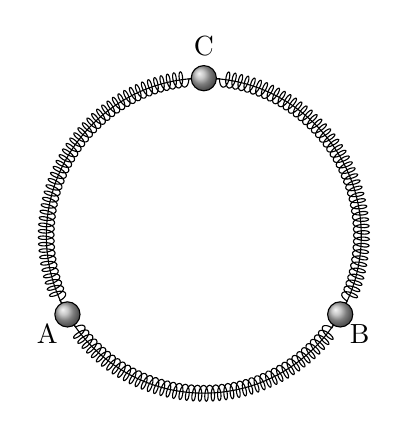
\begin{tikzpicture}
\def\R{2}
\draw (0,0) circle (\R);
\foreach \n in{1,2,3}{
\draw[decorate,decoration={coil,aspect=0.4,amplitude=1mm,segment length=0.8mm,pre length=1.9mm,post length=1.8mm}] ({\R*cos(90+\n*120)},{\R*sin(90+\n*120)}) arc ({90+\n*120}:{90+(\n+1)*120}:\R);}
\foreach \n in{1,2,3}{
\draw[ball color=black!30] ({\R*cos(90+\n*120)},{\R*sin(90+\n*120)}) circle (0.16);}
\node[anchor=north east] at ({\R*cos(90+120)},{\R*sin(90+120)}) {A};
\node[anchor=north west] at ({\R*cos(90+240)},{\R*sin(90+240)}) {B};
\node[above=1.6mm] at ({\R*cos(90)},{\R*sin(90)}) {C};
\end{tikzpicture}
\end{center}
이 시스템의 세 개의 고유모드 중 하나는 A, B, C의 각속도의 비를 열벡터(column vector)로 나타낸
\begin{equation*}
\mathbf{V}_1 =\Omega_1 \begin{pmatrix}1\\1\\1\end{pmatrix}
\end{equation*}
이고, 이 모드의 각진동수는 $\omega_1 =0$이다. 나머지 두 개의 각속도의 고유모드들과 각 모드에 대응하는 고유진동수를 구하시오. (단, 시스템은 원 둘레를 따라서만 운동할 수 있다.)\droppoints

\end{questions}
\end{multicols*}


%%% page 2 %%%
\begin{multicols*}{2}
\begin{questions}\extrawidth{8.1em}\setcounter{question}{2} %이전 페이지 마지막 문항 번호 입력

%%% Prob 3 %%%
\addpoints
\question 다음 물음에 답하시오.\droptotalpoints
\begin{parts}
\part[10] \nsh\ Principal moments of inertia가 $I_x =I_y =I_z$의 관계에 있을 때, 관성 텐서는 질량 중심을 지나는 임의의 직선을 축으로 하는 회전 변환에 대하여 불변임을 보이시오.\droppoints
\vspace{8em}
\part[10] \ssh\ 다음 그림 (가)$\sim$(다)는 질량 $M$, 한 변의 길이가 $b$인 정팔면체를 비틀림 용수철에 매달아 회전 진동을 시키는 모습이다. 각각의 진동 주기를 $T_{(가)}$, $T_{(나)}$, $T_{(다)}$라고 할 때, 진동 주기들의 대소 관계를 구하고, 이유를 설명하시오. (단, 모든 용수철의 비틀림 상수는 동일하다.)\droppoints
\begin{center}
\tdplotsetmaincoords{60}{135}
\begin{tikzpicture}[tdplot_main_coords]
\def\b{1.6}
\draw[line join=bevel,fill=black!4] (0,{-\b/sqrt(2)},0) -- ({\b/sqrt(2)},0,0) -- (0,0,{\b/sqrt(2)}) -- cycle;
\draw[line join=bevel,fill=black!10] ({\b/sqrt(2)},0,0) -- (0,{\b/sqrt(2)},0) -- (0,0,{\b/sqrt(2)}) -- cycle;
\draw[line join=bevel,fill=black!20] (0,{\b/sqrt(2)},0) -- ({-\b/sqrt(2)},0,0) -- (0,0,{\b/sqrt(2)}) -- cycle;
\draw[line join=bevel,fill=black!30] ({\b/sqrt(2)},0,0) -- (0,{\b/sqrt(2)},0) -- (0,0,{-\b/sqrt(2)}) -- cycle;
\draw[thick] (0,0,{\b/sqrt(2)}) -- ++(0,0,{0.4*\b});
\draw[thick] (0,0,{-\b/sqrt(2)}) -- ++(0,0,{-0.3*\b}) node[pos=1,below]{(가)};
\tdplotdrawarc[{Latex[length=1mm]}-{Latex[length=1mm]},thin]{(0,0,{0.3*\b})}{0.6*\b}{-100}{190}{}{}
\end{tikzpicture}
\hspace{2em}
\tdplotsetmaincoords{70}{90}
\begin{tikzpicture}[tdplot_main_coords]
\def\b{1.6}
\draw[line join=bevel,fill=black!4] (0,{-\b/2},{\b/2}) -- ({\b/sqrt(2)},0,0) -- (0,{\b/2},{\b/2}) -- cycle;
\draw[line join=bevel,fill=black!10] (0,{-\b/2},{\b/2}) -- ({\b/sqrt(2)},0,0) -- (0,{-\b/2},{-\b/2}) -- cycle;
\draw[line join=bevel,fill=black!20] (0,{\b/2},{\b/2}) -- ({\b/sqrt(2)},0,0) -- (0,{\b/2},{-\b/2}) -- cycle;
\draw[line join=bevel,fill=black!30] (0,{\b/2},{-\b/2}) -- ({\b/sqrt(2)},0,0) -- (0,{-\b/2},{-\b/2}) -- cycle;
\draw[thick] (0,0,{\b/2}) -- ++(0,0,{0.5*\b});
\draw[thick] (0,0,{-\b/2}) -- ++(0,0,{-0.4*\b}) node[pos=1,below]{(나)};
\tdplotdrawarc[{Latex[length=1mm]}-{Latex[length=1mm]},thin]{(0,0,{0.4*\b})}{0.6*\b}{-165}{165}{}{}
\end{tikzpicture}
\hspace{2em}
\tdplotsetmaincoords{110}{90}
\begin{tikzpicture}[tdplot_main_coords]
\def\b{1.6}
\draw[line join=bevel,fill=black!4] (0,{-\b/2},{\b/2}) -- ({\b/sqrt(2)},0,0) -- (0,{\b/2},{\b/2}) -- cycle;
\draw[line join=bevel,fill=black!10] (0,{-\b/2},{\b/2}) -- ({\b/sqrt(2)},0,0) -- (0,{-\b/2},{-\b/2}) -- cycle;
\draw[line join=bevel,fill=black!20] (0,{\b/2},{\b/2}) -- ({\b/sqrt(2)},0,0) -- (0,{\b/2},{-\b/2}) -- cycle;
\draw[line join=bevel,fill=black!30] (0,{\b/2},{-\b/2}) -- ({\b/sqrt(2)},0,0) -- (0,{-\b/2},{-\b/2}) -- cycle;
\draw[thick] ({-\b/sqrt(2)/3},0,{\b/2}) -- ++(0,0,{0.5*\b});
\draw[thick] (0,0,{-\b/2}) -- ++(0,0,{-0.4*\b}) node[pos=1,below]{(다)};
\tdplotdrawarc[{Latex[length=1mm]}-{Latex[length=1mm]},thin]{(0,0,{0.4*\b})}{0.6*\b}{155}{-155}{}{}
\end{tikzpicture}
\end{center}

\end{parts}

\vspace*{\fill}
\columnbreak

\end{questions}
\end{multicols*}


\end{document}